\section{Implementing a Synchronous Channel}

Conditions can also be used to implement synchronisation objects.  A thread
that needs to synchronise can wait for another thread; when another thread
arrives, it can signal to the waiting thread.  We illustrate the technique by
implementing a basic synchronous channel, to extend the trait in
Figure~\ref{fig:SyncChanT}, with |send| and |receive| operations
that synchronise together.  The channel can be used by an arbitrary number of
senders and receivers.

%%%%%

\begin{figure}
\begin{scala}
trait SyncChanT[A]{
  /** Send £x£, synchronously. */
  def send(x: A): Unit

  /** Receive a value. */
  def receive(): A
}
\end{scala}
\caption{The trait for a synchronous channel.}
\label{fig:SyncChanT}
\end{figure}

%%%%%

The implementation is in Figure~\ref{fig:SharedSyncChan}.  The variable
|value| holds the value currently being sent, or maybe the previous value
sent.  The variable |full| indicates whether the value in |value| is valid,
i.e.~if a current sender is trying to send it. 

%%%%% Check positioning of figure.

\begin{figure}
\begin{center}
\def\height{5.7}
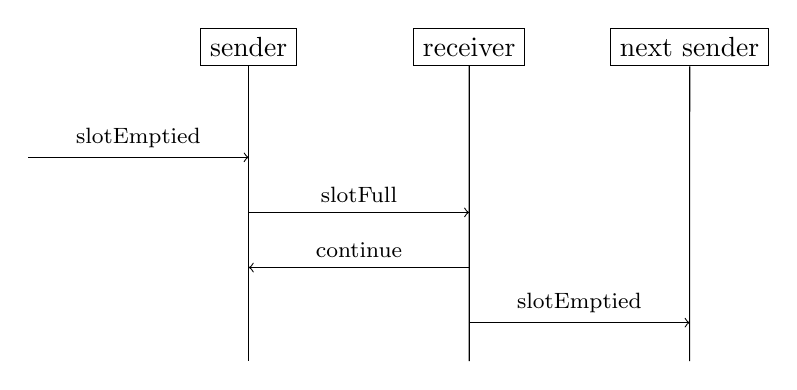
\begin{tikzpicture}[xscale = 2.8, yscale = 0.7]
\draw (0,0) node[draw] (sender) {sender};
\draw (sender) -- ++ (0,-\height);
\draw (1,0) node[draw] (receiver) {receiver}; 
\draw (receiver) -- ++ (0,-\height);
\draw (2,0) node[draw] (sender2) {next sender};
\draw (sender2) -- ++ (0,-\height);
%
\draw[<-] (sender) ++ (0,-2) -- 
  node[above]{\scalashape\footnotesize slotEmptied} ++ (-1,0); 
\draw[->] (sender) ++ (0,-3) -- 
  node[above]{\scalashape\footnotesize slotFull} ++ (1,0);
\draw[->] (receiver) ++ (0,-4) --
  node[above]{\scalashape\footnotesize continue} ++ (-1,0);
\draw[->] (receiver) ++ (0,-5) --
  node[above]{\scalashape\footnotesize slotEmptied} ++ (1,0);
\end{tikzpicture}
\end{center}
\caption{A sequence diagram illustrating the signals in the implementation of
  a synchronous channel.}
\label{fig:syncChan-seqDiagram}
\end{figure}

%%%%%

\begin{figure}
\begin{scala}
class SharedSyncChan[A] extends SyncChanT[A]{
  /** The current or previous value. */
  private var value = null.asInstanceOf[A]

  /** Is the current value of £value£ valid, i.e. ready to be received? */
  private var full = false

  /** Monitor for controlling synchronisations. */
  private val lock = new Lock

  /** Condition for signalling to sender that a value has been deposited. */
  private val slotFull = lock.newCondition

  /** Condition for signalling to current receiver that it can continue. */
  private val continue = lock.newCondition

  /** Condition for signalling to the next sender that the previous value has
    * been read. */
  private val slotEmptied = lock.newCondition

  def send(x: A) = lock.mutex{
    slotEmptied.await(!full) // Wait for previous value to be consumed (1).
    value = x; full = true   // Deposit my value.
    slotFull.signal()        // Signal to receiver at (2).
    continue.await()         // Wait for receiver (3).
  }

  def receive(): A = lock.mutex{
    slotFull.await(full)               // Wait for sender (2).
    continue.signal()                  // Notify current sender at (3).
    full = false                       // Clear the slot.
    slotEmptied.signal() // Clear value, and notify next sender at (1).
    value
  }
}
\end{scala}
\caption{The implementation of a synchronous channel.}
\label{fig:SharedSyncChan}
\end{figure}

%%%%%

We require three conditions for signals between threads:
%
\begin{itemize}
\item Each sender will signal to a receiver on |slotFull| that it has
  deposited a value, which the receiver can take;

\item The receiver will then signal back to the sender on |continue| that it
  can continue; this makes the channel synchronous;

\item The receiver will signal to a sender for the next round on |slotEmptied|
  that it has cleared the value, so that sender can deposit its value.
\end{itemize}
%
Figure~\ref{fig:syncChan-seqDiagram} illustrates the sequence of signals.

The sender waits, on |slotEmptied|, until the previous exchange is complete.
Note that it needs to recheck |full| when it receives a signal on, in case
another sender has run in the meantime and filled the slot.  It then deposits
its value, and signals to a waiting receiver on |slotFull|.  Finally, it waits
for a signal back on |continue|.  Note that there is no need to recheck |full|
at this point, as it cannot be preempted by another sender. 

The receiver waits, on |slotFull|, for a value to be deposited.  It again
needs to recheck |full| when it receives a signal, in case another receiver
has run in the meantime and taken the value.  It then signals back to the
sender on |continue|, clears the slot, and then signals to the next sender on
|slotEmptied|. 

\begin{instruction}
Study the details of the implementation.  Make sure you understand why each of
the signals is necessary.
\end{instruction}


We can test this implementation by running some threads that perform sends and
receives, and log the call and return of each operation.  For simplicity, we
arrange that every send is of a different value.  This makes it easy to
identify matching sends and receives (if they exist).  We then check that the
two invocations overlap.  

As in Section~\ref{sec:exchanger}, it is sound to assume the values sent are
all different, because the implementation is \emph{data independent} in the
type |A| of data: values of this type are stored, read, and returned, but no
operation (e.g.~|==|) is done on them.  This means that for any erroneous
history, there would be a corresponding erroneous history using distinct
values.

